\section{Method}
%La rete è stata implementata su python 3.8 facendo uso delle seguenti librerie:
The network was implemented on python 3.8 with the help, mainly, of the following libraries:
\begin{itemize}
    %\item numpy, per le operazioni di algebra lineare, di cui abbiamo fatto ampio uso, e per la gestione degli array multidimensionali;
    \item numpy, for linear algebra operations, which we used a lot, and for the multidimensional arrays management;
    \item matplotlib.pyplot, to build the plots;
    \item sklearn.modelselection, only the subroutines that manage the k-fold creation.
\end{itemize}
The library we built consists of classes that allow the construction and management of the network (training, cross-validation on the development set etc...). The \textit{Layer} represents a layer (hidden or output) of the network and implements the node values (those generated by the activation function), weights, deltas and gradients; the \textit{NeuralNetwork} class builds the hidden and output layers given the structure of the network and the activation functions of each layer: sigmoidal \textit{Sigmoid($\alpha$)}, hyperbolic tangent \textit{TanH()}, \textit{LeakyReLU()} and \textit{Linear($\alpha$)}; then the nodes are created with their weights chosen randomly in the range $[\frac{-0.7*fan-in}{2}, \frac{0.7*fan-in}{2}]$. The $\alpha$ parameter in \textit{Linear} is the angular coefficient of the straight, while $\alpha=1$ in \textit{Sigmoid} represents the logistic function. The \textit{NeuralNetwork} class defines the \textit{train} method that, as the name says, trains the network given a set of hyper-parameters and a Loss function, once the method ends it returns the average errors on the training and validation set; if we're dealing with a classification task, the \textit{train} method also returns the accuracy on the training and validation sets. The \textit{train} method is, in fact, the heart of our library since it implements the main functions (using many submethods): feed forward, back-propagation (only based on the MSE for time and simplicity reasons, based on what we've seen in the Haykin book\cite{haykin2009neural}) and updates the weights at the end of each batch.
%La libreria è composta da una classe \textit{Layer} che contiene i valori dei nodi, i loro relativi pesi, delta ed i gradienti. La classe \textit{NeuralNetwok} data la struttura della rete, e le funzioni di attivazione, crea gli hidden e output \textit{Layer}. Le funzioni di attivazione implementate sono la sigmoidal \textit{Sigmoid($\alpha$)}, hyperbolic tangent \textit{TanH()}, \textit{LeakyReLU()} e \textit{Linear()}  In seguito vengono creati i nodi ed i relativi pesi, presi nell'insieme $[\frac{-0.7*fan-in}{2}, \frac{0.7*fan-in}{2}]$. Nella classe \textit{NeuralNetwok}, è stato implementato il metodo \textit{train}, che allena la rete neurale secondo degli hyperparameters e data una Cost function, restituisce gli errori medi nel training set e nel validation set. Nel caso trattassimo un problema di classificazione, restituisce anche l'accuracy calcolata nel training e nel validation set. Il metodo \textit{train} fa il feed forward e ed aggiorna i pesi dei nodi applicando la backpropagation. Nel progetto sono stati implementati tutti i metodi per il calcolo della discesa del gradiente ossia stocastico, mini-batch e batch (full). Nel caso in cui non si applichi il metodo batch, viene utilizzato \textit{adaptive learning rate}.\\
\vspace{3mm}

The \textit{GridSearchCV} class takes care of the selection phase of the best hyperparameters by combining grid search with k-fold cross validation. Given a set of hyperparameters, k (\# of folds) and Cost Function, it applies k-fold cross validation to each combination of hyperparameters and calculates the average training and validation error in the k-folds, in order to select the best model. The hyperparameters on which the grid search can be applied are: the network structure (number of hidden layers and nodes), learning rate, Nesterov momentum, Tikhonov regularization (weight decay) and batch size. The activation functions have not been included in the hyperparameters because a pre-test was made before the grid search, in order to understand which one was the best, based on the smoothness of the learning curve and the error on the validation set.
%La classe \textit{GridSearchCV} si occupa della fase di selezione dei migliori iperparamentri combinando la grid search con la k-fold cross validation. Dati un set di iperparametri, un k e Cost Function, applica la k-fold cross validation ad ogni combinazione di iperparametri e calcola l'errore medio di training e di validation nei k-fold, al fine di selezionare il modello migliore. Gli hyperparameters su cui è possibile applicare la grid search sono: la struttura della rete (numero di hidden layer e nodi), il learning rate, il Nesterov momentum, il weight decay ed il batch size. Le funzioni di attivazione non sono state inserite negli iperparamentri perché prima della grid search è stato fatto un pre-test per capire quale fosse la migliore, in base alla smoothness della curva di apprendimento ed all'errore sul validation set.

\subsection{Preprocessing}
Inside the library there is a \textit{Utilities} class that does the preprocessing work. In the MONKS dataset, after reading the training and test files, it applies 1-k encoding on the inputs. In the CUP data set, it partitions the ML-CUP20-TR.csv set in such a way as to obtain two independent sets: the development set (on which we apply the cross-validation), that consists of the training and validation set, and the (internal) test set. Further details on partitioning has been described in \ref{subsec:cupResult}. For both MONKS and CUP, the entire development dataset has been divided into inputs and targets.
%All'interno della libreria è presente una classe \textit{Utilities} che svolge il lavoro di preprocessing. Per quanto riguarda i MONKS, dopo aver letto i file di training e test, applica la 1-k encoding sugli input. Per quanto riguarda la CUP invece, partiziona il training set in modo tale da ottenere due set indipendenti, cioè il training set compreso di validation set ed il test set (interno). Il partizionamento preciso è stato descritto in \ref{subsec:cupResult}. Sia per i MONKS che per la CUP, l'intero data set di training è stato diviso in input e target.

%\begin{figure}[h]
%\centering
%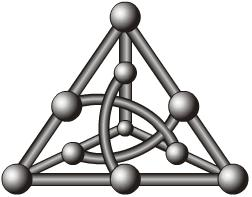
\includegraphics[width=0.3\textwidth]{figure.jpg}
%\caption{Do \textit{not} insert a picture of your network (unless innovative).}
%\label{fig:myfigure}
%\end{figure}
%\newpage